Fold back on dotted lines and forward on dashed lines. \medskip

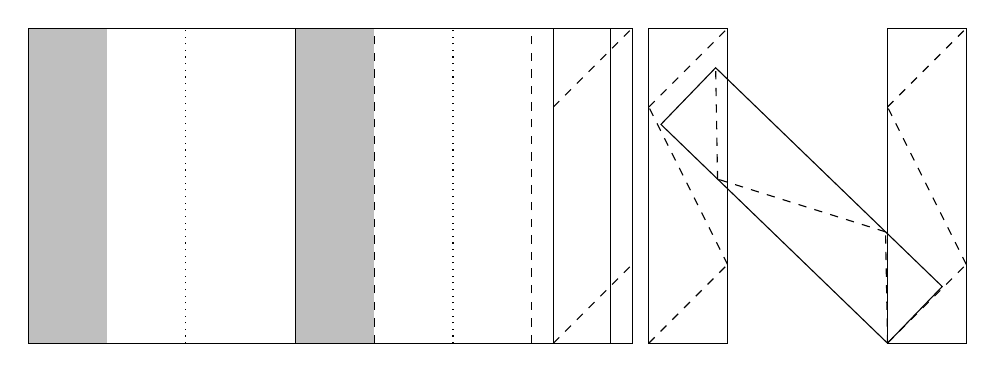
\begin{tikzpicture}
	\begin{scope}
	\draw[fill=lightgray, draw=none] (0,0) --(1,0) -- (1,4) -- (0,4) -- cycle;
		\draw (0,0) -- (4,0) -- (4,4) -- (0,4) -- cycle;
	\draw[dotted] (2,0) -- (2,4);
	\end{scope}
	
	\begin{scope}[xshift=.28\textwidth]
	\draw[fill=lightgray, draw=none] (0,0) --(1,0) -- (1,4) -- (0,4) -- cycle;
		\draw (0,0) -- (4,0) -- (4,4) -- (0,4) -- cycle;
	\draw[dotted] (2,0) -- (2,4);
\draw[dashed] (1,0) -- (1,4);
	\draw[dashed] (3,0) -- (3,4);
		
	\end{scope}
	
	\begin{scope}[xshift=.55\textwidth]
		\draw[] (0,0) --(1,0) -- (1,4) -- (0,4) -- cycle;
		\draw[dashed] (0,0) -- (1,1);
		\draw[dashed] (0,3) -- (1,4);
	\end{scope}

\begin{scope}[xshift = .65\textwidth]
		\draw[] (0,0) --(1,0) -- (1,4) -- (0,4) -- cycle;
		\draw[dashed] (0,0) -- (1,1);
		\draw[dashed] (0,3) -- (1,4);
		\draw[dashed] (1,1) -- (0,3);
	\end{scope}
	
	\begin{scope}[xshift=.9\textwidth]
			\begin{scope}
		\draw[] (0,0) --(1,0) -- (1,4) -- (0,4) -- cycle;
		\draw[dashed] (0,0) -- (1,1);
		\draw[dashed] (0,3) -- (1,4);
		\draw[dashed] (1,1) -- (0,3);
	\end{scope}
	
	\begin{scope}[rotate=46]
		\draw[] (0,0) --(1,0) -- (1,4) -- (0,4) -- cycle;
		\draw[dashed] (0,0) -- (1,1);
		\draw[dashed] (0,3) -- (1,4);
		\draw[dashed] (1,1) -- (0,3);
	\end{scope}

	\end{scope}
\end{tikzpicture}

\vfill

Fold back on dotted lines and forward on dashed lines. \medskip

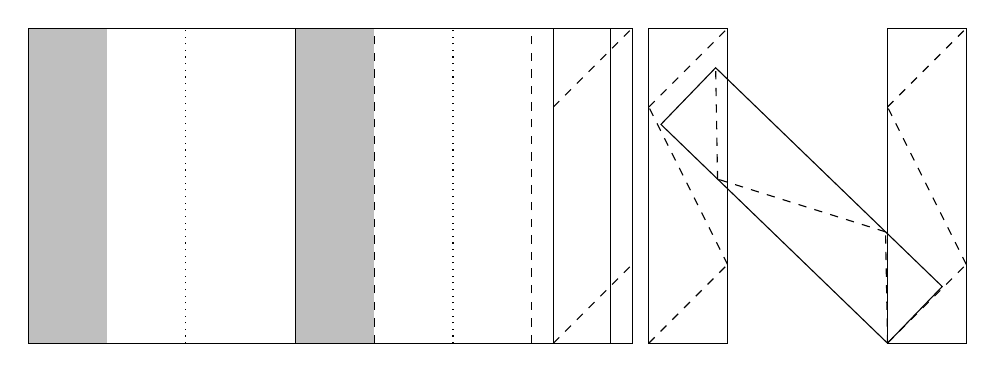
\begin{tikzpicture}
	\begin{scope}
	\draw[fill=lightgray, draw=none] (0,0) --(1,0) -- (1,4) -- (0,4) -- cycle;
		\draw (0,0) -- (4,0) -- (4,4) -- (0,4) -- cycle;
	\draw[dotted] (2,0) -- (2,4);
	\end{scope}
	
	\begin{scope}[xshift=.28\textwidth]
	\draw[fill=lightgray, draw=none] (0,0) --(1,0) -- (1,4) -- (0,4) -- cycle;
		\draw (0,0) -- (4,0) -- (4,4) -- (0,4) -- cycle;
	\draw[dotted] (2,0) -- (2,4);
\draw[dashed] (1,0) -- (1,4);
	\draw[dashed] (3,0) -- (3,4);
		
	\end{scope}
	
	\begin{scope}[xshift=.55\textwidth]
		\draw[] (0,0) --(1,0) -- (1,4) -- (0,4) -- cycle;
		\draw[dashed] (0,0) -- (1,1);
		\draw[dashed] (0,3) -- (1,4);
	\end{scope}

\begin{scope}[xshift = .65\textwidth]
		\draw[] (0,0) --(1,0) -- (1,4) -- (0,4) -- cycle;
		\draw[dashed] (0,0) -- (1,1);
		\draw[dashed] (0,3) -- (1,4);
		\draw[dashed] (1,1) -- (0,3);
	\end{scope}
	
	\begin{scope}[xshift=.9\textwidth]
			\begin{scope}
		\draw[] (0,0) --(1,0) -- (1,4) -- (0,4) -- cycle;
		\draw[dashed] (0,0) -- (1,1);
		\draw[dashed] (0,3) -- (1,4);
		\draw[dashed] (1,1) -- (0,3);
	\end{scope}
	
	\begin{scope}[rotate=46]
		\draw[] (0,0) --(1,0) -- (1,4) -- (0,4) -- cycle;
		\draw[dashed] (0,0) -- (1,1);
		\draw[dashed] (0,3) -- (1,4);
		\draw[dashed] (1,1) -- (0,3);
	\end{scope}

	\end{scope}
\end{tikzpicture}



\vfill

Fold back on dotted lines and forward on dashed lines. \medskip

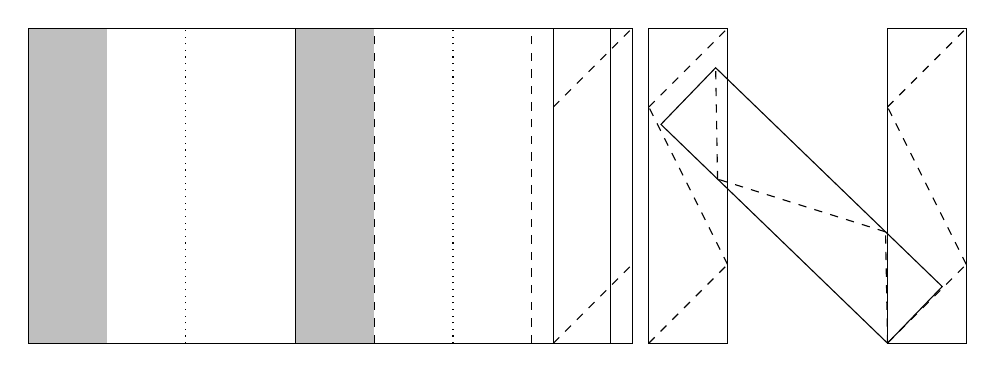
\begin{tikzpicture}
	\begin{scope}
	\draw[fill=lightgray, draw=none] (0,0) --(1,0) -- (1,4) -- (0,4) -- cycle;
		\draw (0,0) -- (4,0) -- (4,4) -- (0,4) -- cycle;
	\draw[dotted] (2,0) -- (2,4);
	\end{scope}
	
	\begin{scope}[xshift=.28\textwidth]
	\draw[fill=lightgray, draw=none] (0,0) --(1,0) -- (1,4) -- (0,4) -- cycle;
		\draw (0,0) -- (4,0) -- (4,4) -- (0,4) -- cycle;
	\draw[dotted] (2,0) -- (2,4);
\draw[dashed] (1,0) -- (1,4);
	\draw[dashed] (3,0) -- (3,4);
		
	\end{scope}
	
	\begin{scope}[xshift=.55\textwidth]
		\draw[] (0,0) --(1,0) -- (1,4) -- (0,4) -- cycle;
		\draw[dashed] (0,0) -- (1,1);
		\draw[dashed] (0,3) -- (1,4);
	\end{scope}

\begin{scope}[xshift = .65\textwidth]
		\draw[] (0,0) --(1,0) -- (1,4) -- (0,4) -- cycle;
		\draw[dashed] (0,0) -- (1,1);
		\draw[dashed] (0,3) -- (1,4);
		\draw[dashed] (1,1) -- (0,3);
	\end{scope}
	
	\begin{scope}[xshift=.9\textwidth]
		\draw[] (0,0) --(1,0) -- (1,4) -- (0,4) -- cycle;
		\draw[dashed] (0,0) -- (1,1);
		\draw[dashed] (0,3) -- (1,4);
		\draw[dashed] (1,1) -- (0,3);
	
		\begin{scope}[rotate=46]
		\draw[] (0,0) --(1,0) -- (1,4) -- (0,4) -- cycle;
		\draw[dashed] (0,0) -- (1,1);
		\draw[dashed] (0,3) -- (1,4);
		\draw[dashed] (1,1) -- (0,3);
	\end{scope}

	\end{scope}
\end{tikzpicture}

